%%%%%%%%%%%%%%%%%%%%%%%%%%%%%%%%%%%%%%%%%%%%%%%%%%%%%%%%%%%%%%%%%%%%%%%%%%%%%
% 26/05/2010
% edited by Bill Lampos
%
% Feel free to use (copy) the structure (latex formatting source code)
% but not the content of this document.
%
%%%%%%%%%%%%%%%%%%%%%%%%%%%%%%%%%%%%%%%%%%%%%%%%%%%%%%%%%%%%%%%%%%%%%%%%%%%%%
\documentclass[compress,red]{beamer}
\mode<presentation>

\usetheme{Warsaw}
%\usetheme{Darmstadt}
% other themes: AnnArbor, Antibes, Bergen, Berkeley, Berlin, Boadilla, boxes, CambridgeUS, Copenhagen, Darmstadt, default, Dresden, Frankfurt, Goettingen,
% Hannover, Ilmenau, JuanLesPins, Luebeck, Madrid, Maloe, Marburg, Montpellier, PaloAlto, Pittsburg, Rochester, Singapore, Szeged, classic

%\usecolortheme{lily}
% color themes: albatross, beaver, beetle, crane, default, dolphin, dov, fly, lily, orchid, rose, seagull, seahorse, sidebartab, structure, whale, wolverine

%\usefonttheme{serif}
% font themes: default, professionalfonts, serif, structurebold, structureitalicserif, structuresmallcapsserif

% pdf is displayed in full screen mode automatically
%\hypersetup{pdfpagemode=FullScreen}

% define your own colours:
\definecolor{Red}{rgb}{1,0,0}
\definecolor{Blue}{rgb}{0,0,1}
\definecolor{Green}{rgb}{0,1,0}
\definecolor{magenta}{rgb}{1,0,.6}
\definecolor{lightblue}{rgb}{0,.5,1}
\definecolor{lightpurple}{rgb}{.6,.4,1}
\definecolor{gold}{rgb}{.6,.5,0}
\definecolor{orange}{rgb}{1,0.4,0}
\definecolor{hotpink}{rgb}{1,0,0.5}
\definecolor{newcolor2}{rgb}{.5,.3,.5}
\definecolor{newcolor}{rgb}{0,.3,1}
\definecolor{newcolor3}{rgb}{1,0,.35}
\definecolor{darkgreen1}{rgb}{0, .35, 0}
\definecolor{darkgreen}{rgb}{0, .6, 0}
\definecolor{darkred}{rgb}{.75,0,0}

\xdefinecolor{olive}{cmyk}{0.64,0,0.95,0.4}
\xdefinecolor{purpleish}{cmyk}{0.75,0.75,0,0}

% \usepackage{beamerinnertheme_______}
% inner themes include circles, default, inmargin, rectangles, rounded

%\usepackage{beamerouterthemesmoothbars}
% outer themes include default, infolines, miniframes, shadow, sidebar, smoothbars, smoothtree, split, tree

\useoutertheme[subsection=false]{smoothbars}

% to have the same footer on all slides
%\setbeamertemplate{footline}[text line]{xxx xxx xxx}
%\setbeamertemplate{footline}[text line]{} % or empty footer

% include packages
\usepackage{subfigure}
\usepackage{multicol}
\usepackage{amsmath}
\usepackage{epsfig}
\usepackage{graphicx}
\usepackage[all,knot]{xy}
\xyoption{arc}
\usepackage{url}
\usepackage{multimedia}
\usepackage{hyperref}
\usepackage{setspace}
%Page number
%\setbeamertemplate{footline}[frame number]
\setbeamertemplate{sidebar right}{}
\setbeamertemplate{footline}{%
\hfill\usebeamertemplate***{navigation symbols}
\hspace{1cm}\insertframenumber{}/\inserttotalframenumber}

\title{$3^{rd}$ Ph.D. Review}
\subtitle{Tracking trends on the web using novel Machine Learning methods}
\author{Vasileios Lampos}
\institute{{\tiny advised by}\\ \vspace{.10cm}Professor Nello Cristianini}
\date{\scriptsize Intelligent Systems Laboratory, University of Bristol\\ \vspace{.10cm}May 25, 2010}

\begin{document}

\frame{
	\titlepage
}

\section[Outline]{}
\frame{\tableofcontents}

\section{General overview of the project}
\subsection{Aims}
\frame{\frametitle{Aims}
The \textbf{general aims} of our research project can be summarised in the following points:
\vspace{0.25cm}
\begin{enumerate}
\item Track \textbf{trends} on the Web by applying Machine Learning methods (track expresses the notions of infer or predict as well)
\vspace{0.25cm}
\item Extend current or invent new \textbf{methodologies} (where and if needed) for accomplishing our primary aim
\vspace{0.25cm}
\item Build \textbf{tools} that apply the experimental/theoretical results in real and large-scale applications (featured research)
\end{enumerate}
}

\subsection{Being more specific}
\frame{\frametitle{Being more specific}
\begin{enumerate}
\item \textbf{Trends} about what? Examples?
      \begin{itemize}
        \item Predict flu rates (\emph{epidemics})
        \item Infer vote intensions (\emph{politics})
        \item Infer traffic/weather conditions (\emph{toy problems})\pause
      \end{itemize}
\vspace{0.25cm}
\item \textbf{Methodologies}?
      \begin{itemize}
        \item Feature extraction/selection
        \item Exploit probabilistic relationships (PGMs)
        \item Regression/classification/ranking scenarios
        \item Active learning\pause
      \end{itemize}
\vspace{0.25cm}
\item \textbf{Applications}?
      \begin{itemize}
        \item Back-end infrastructure for data collection/retrieval/mining
        \item Real time online tools for making and displaying predictions (like the \href{http://geopatterns.enm.bris.ac.uk/epidemics/}{\textbf{Flu detector}})
      \end{itemize}
\end{enumerate}
}

\section{Last 6 months}
\subsection{P1: Tracking the flu pandemic by monitoring the Social Web}
\frame{\frametitle{P1 - Summary (1 of 3)}
{\footnotesize
\begin{tabbing}
Title: \hspace{1.25cm} \= \textbf{Tracking the flu pandemic by monitoring the Social Web}\\
Authors:               \> V. Lampos and N. Cristianini\\
Submitted to:          \> IAPR Cognitive Information Processing 2010 (accepted)
\end{tabbing}
}
\begin{itemize}
\item Twitter and Health Protection Agency data for weeks 26-49, 2009 (on average 160,000 tweets collected per day geolocated in 54 urban centres in the UK)
\item Frequency of \textbf{41 flu related words} (markers) in Twitter corpus had a correlation of $>$\textbf{80\%} with the HPA flu rates in all UK regions
\item Learn a better list of weighted markers \textbf{automatically}:
    \begin{itemize}
    \item Generate a list of candidate markers (1560 words taken from flu related web pages)
    \item Use \textbf{LASSO} for feature selection
    \end{itemize}
\end{itemize}
}

\frame{\frametitle{P1 - Summary (2 of 3)}

\textbf{Validation} schemes:
    \begin{enumerate}
    \item Train on one region, validate regularisation parameter on another, test on the remaining regions (for all possible combinations)

    \begin{table}[!t]
    \tiny
    \renewcommand{\arraystretch}{1}
    \centering
    \begin{tabular}{cccccc}
    \hline
    Train/Validate (regions) & \textbf{A} & \textbf{B}      & \textbf{C} & \textbf{D}       & \textbf{E}     \\\hline
    \textbf{A}     & -          & 0.9594          & 0.9375     & 0.9348           & 0.9297         \\%\hline
    \textbf{B}     & 0.9455     & -               & 0.9476     & 0.9267           & 0.9003         \\%\hline
    \textbf{C}     & 0.9154     & 0.9513          & -          & 0.8188           & 0.908          \\%\hline
    \textbf{D}     & 0.9463     & 0.9459          & 0.9424     & -                & 0.9337         \\%\hline
    \textbf{E}     & 0.8798     & 0.9506          & 0.9455     & 0.8935           & -              \\\hline
    &              &            &\multicolumn{2}{c}{Total Avg.}                   & \textbf{0.9256}\\\cline{4-6}
    \end{tabular}
    \end{table}

    \begin{spacing}{0.5}{
    \textbf{97 selected words}\tiny : lung, unwel, temperatur, like, headach, season, unusu, chronic, child, dai, appetit, stai, symptom, spread, diarrhoea, start, muscl, weaken, immun, feel, liver, plenti, antivir, follow,
    sore, peopl, nation, small, pandem, pregnant, thermomet, bed, loss, heart, mention, condit, ...
    }
    \end{spacing}

    \item Aggregate data from all regions, test on weeks 28 and 41 (2009) and train using the rest of the data set
    \end{enumerate}
}

\frame{\frametitle{P1 - Summary (3 of 3)}
\begin{enumerate}
\item Inferred vs Official flu rate in North England\\
\centering 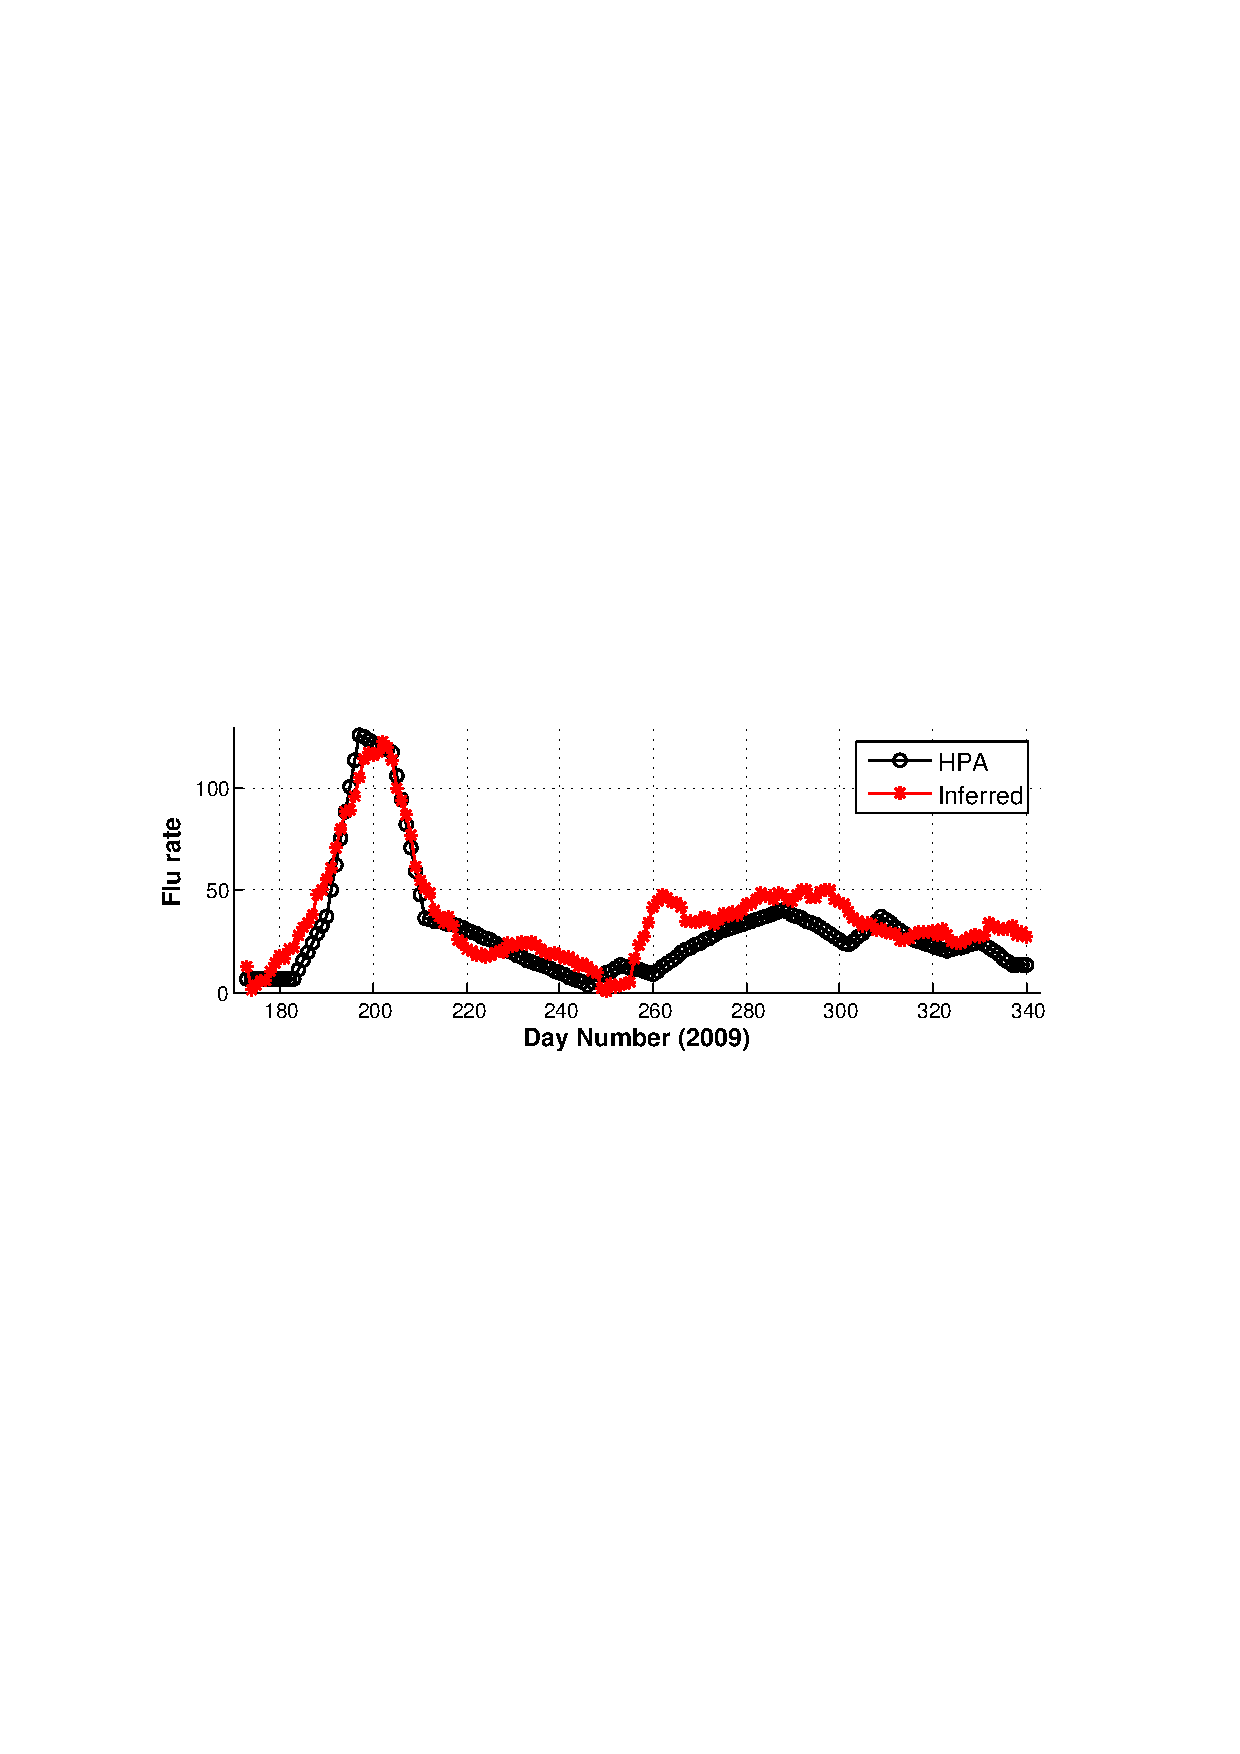
\includegraphics[scale=.5]{figures/Lasso_Inference_regionC_NEng.pdf}

\item Inferred vs Official rates in all regions (aggregated data set)\\
\centering 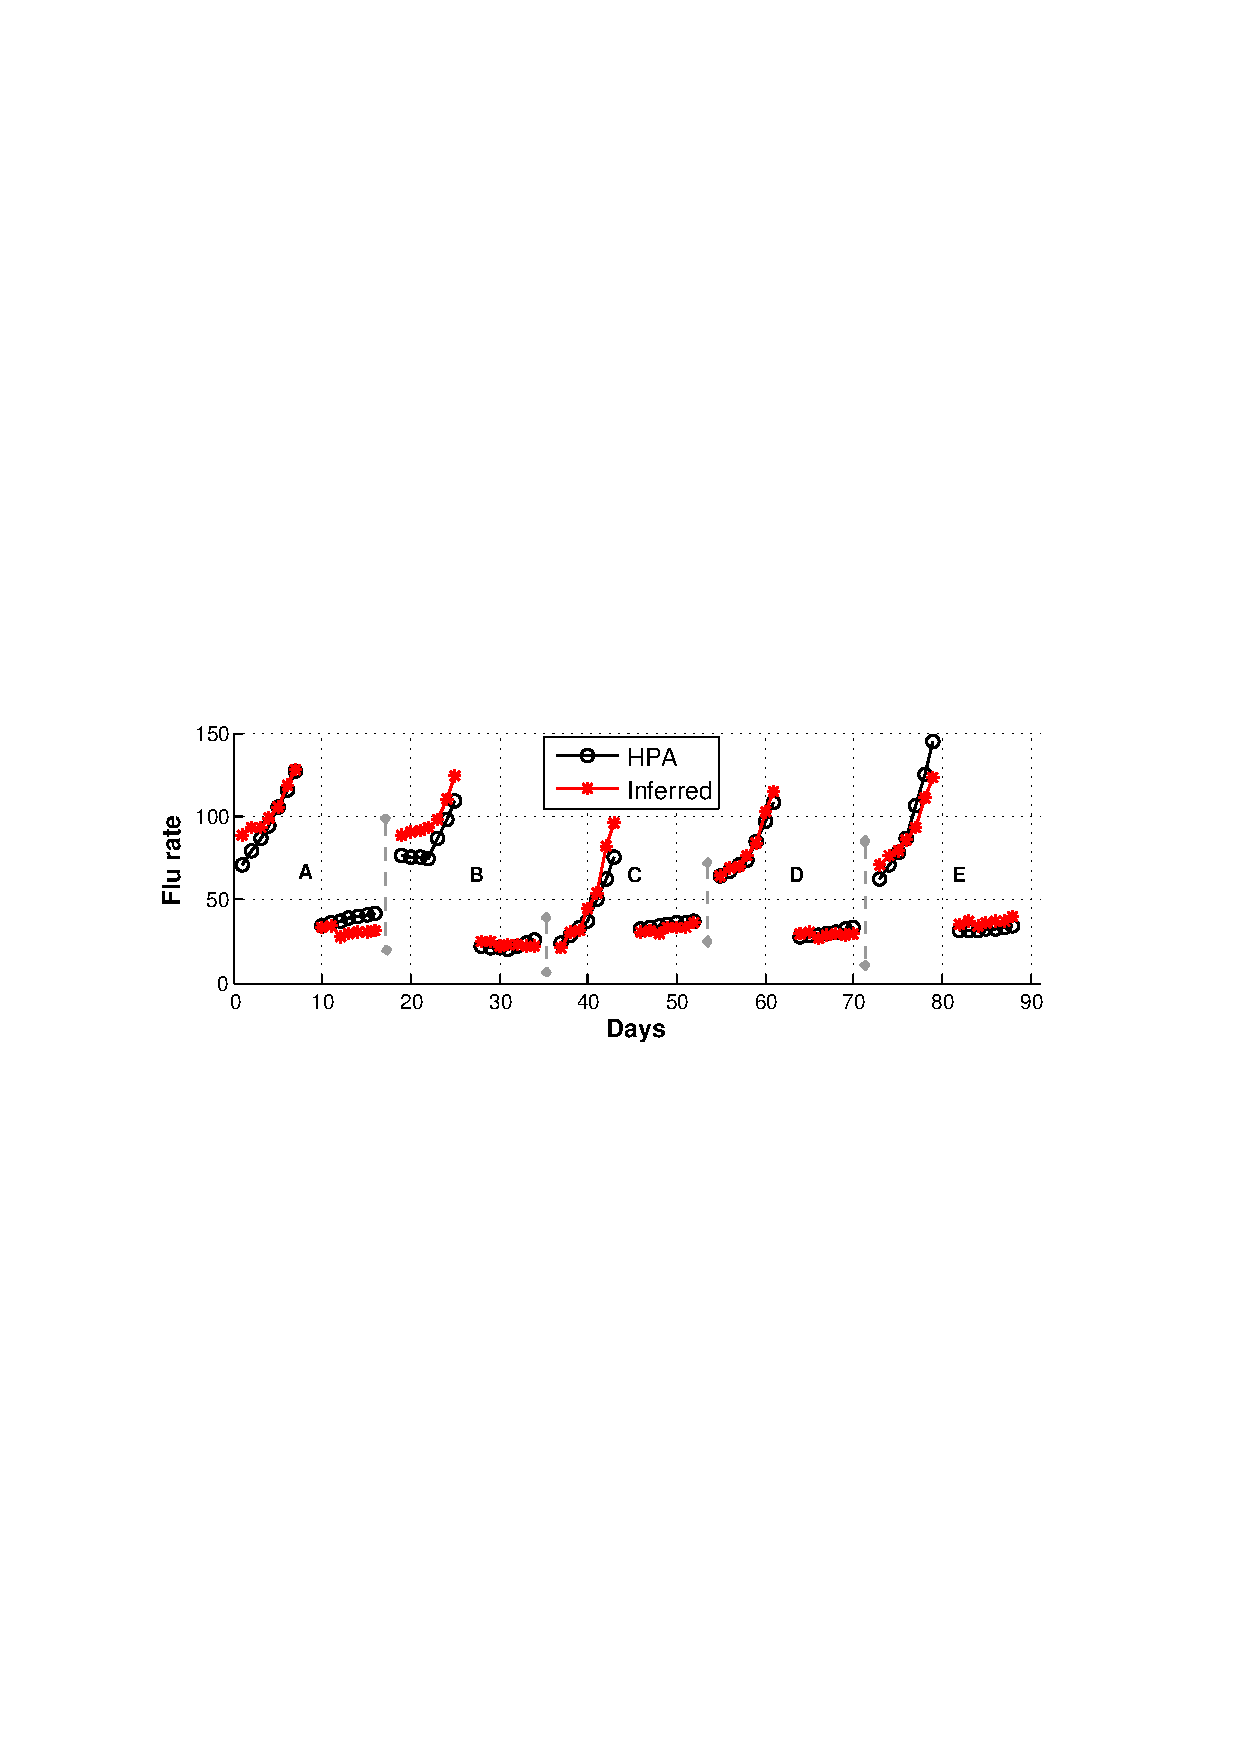
\includegraphics[scale=.5]{figures/Lasso_Inference_Aggregate_IMPROVED.pdf}

\end{enumerate}
}

\subsection{P2: Flu detector - Tracking epidemics on Twitter}
\frame{\frametitle{P2 - Summary}
{\footnotesize
\begin{tabbing}
Title: \hspace{1.25cm} \= \textbf{Flu detector - Tracking epidemics on Twitter}\\
Authors:               \> V. Lampos, T. De Bie, and N. Cristianini\\
Submitted to:          \> ECML PKDD 2010 Demos (under review)
\end{tabbing}
}

\begin{itemize}
\item Extending and making more robust the methodology of P1
\item Larger data sets (bigger time series) and more (2675) \href{http://geopatterns.enm.bris.ac.uk/epidemics/files/candidate_features.txt}{candidate features}
\item Select a list of features (markers) using BoLASSO (bootstrap version of LASSO)
\item Then learn weights of those markers via linear least squares regression
\item Stricter evaluation of the methodology - \href{http://geopatterns.enm.bris.ac.uk/epidemics/twitter-flu-eval.php}{\textbf{Available online}}
\item Put all this into practice and come up with the \href{http://geopatterns.enm.bris.ac.uk/epidemics/}{\textbf{Flu detector}}
\end{itemize}
}

\subsection{Other activities}
\frame{\frametitle{Other activities}
\begin{itemize}
\item Studied/implemented the necessary statistical tools and algorithms (in MATLAB or Java)
\item Extended further the infrastructure for conducting large scale experiments and data retrieval on demand
\item TA for Intro to AI, Data Analysis and Pattern Analysis \& Statistical Learning
\item Attended some of the ISL meetings and seminars
\end{itemize}
}

\section{Next 6 months}
\subsection{General goals \& activities}
\frame{\frametitle{General goals \& activities}
\begin{enumerate}
\item ... (content omitted)
\item ... (content omitted)
\item ... (content omitted)
\item ... (content omitted)
\end{enumerate}
}

\subsection{A more time specific tentative plan}
\frame{\frametitle{A more time specific tentative plan}
\begin{itemize}
\item In \textbf{June}: ... (content omitted)
\item In \textbf{July}: ... (content omitted)
\item In \textbf{August}: ... (content omitted)
\item In \textbf{September - November}: ... (content omitted)
\end{itemize}
}

\section*{}
\frame{
    \begin{center}
        \huge
        This is the last slide.\\ \pause
        \vspace{1cm}
        Any questions?
    \end{center}
}

\end{document} 